\begin{frame}{Suche am Beispiel Map Coloring}
\begin{center}
\def\svgwidth{.55\columnwidth}
\input{img/australia-large-exp.pdf_tex}
\end{center}

$X = \{ \mathsf{WA}, \mathsf{NT}, \ldots \mathsf{V} \}$, $D_x = \{\mathsf{r}, \mathsf{g}, \mathsf{b} \}$, $C = \{
\mathsf{WA} \neq \mathsf{NT}, \mathsf{NT} \neq \mathsf{SA}, \ldots  \}$


\end{frame}

\begin{frame}{Systematische Suche I}

\begin{center}
\begin{tikzpicture}[auto,
                    ->,>=stealth',shorten >=1pt,thick,
                    node distance=2.7cm,inner sep=0pt,
                    constraint/.style={circle,fill=black!15,draw,font=\sffamily\small}]
\node (1) at (0, 0)                   {
\def\svgwidth{.15\columnwidth}
\input{img/australia.pdf_tex}
};

\node[below of=1] (3) {
\def\svgwidth{.15\columnwidth}
\input{img/wa-red.pdf_tex}
};  

\node[left of=3] (2) {
\def\svgwidth{.15\columnwidth}
\input{img/wa-blue.pdf_tex}
};  


\node[right of=3] (4) {
\def\svgwidth{.15\columnwidth}
\input{img/wa-green.pdf_tex}
};

\path[every node/.style={font=\sffamily\tiny}]
  (1) edge (2)
  (1) edge (3)
  (1) edge (4)
 ;

\node[below left of=2] (5) {
\def\svgwidth{.15\columnwidth}
\input{img/blue-red.pdf_tex}
};

\node[below right of=2] (6) {
\def\svgwidth{.15\columnwidth}
\input{img/blue-green.pdf_tex}
};
%  
\path[every node/.style={font=\sffamily\tiny}]
  (2) edge (5)
  (2) edge (6)
  ;
\end{tikzpicture}
\end{center}
\end{frame}

\begin{frame}{Systematische Suche II}

\begin{center}
\begin{tikzpicture}[auto,
                    ->,>=stealth',shorten >=1pt,thick,
                    node distance=2.7cm,inner sep=0pt,
                    constraint/.style={circle,fill=black!15,draw,font=\sffamily\small}]
\node (1) at (0, 0)                   {
\def\svgwidth{.15\columnwidth}
\input{img/blue-red.pdf_tex}
};

\node[below left of=1] (2) {
\def\svgwidth{.15\columnwidth}
\input{img/wa-red-green.pdf_tex}

{\huge
\alert{\Lightning}
}
};  

\node[below right of=1] (3) {
\def\svgwidth{.15\columnwidth}
\input{img/wa-red-blue.pdf_tex}
};  

\path[every node/.style={font=\sffamily\tiny}]
  (1) edge (2)
  (1) edge (3)
 ;

\node[below of=3] (5) {
\def\svgwidth{.15\columnwidth}
\input{img/wa-red-green-blue.pdf_tex}
};
%  
\path[every node/.style={font=\sffamily\tiny}]
  (3) edge (5)
  ;
\end{tikzpicture}
\end{center}

\end{frame}

\begin{frame}{Tricks (Heuristiken)}
Wähle Länder (Variablen) und Farben (Werte) in \alert{geschickter} Reihenfolge aus


\begin{itemize}
\item \emph{Minimum-Remaining-Values} (MRV): Wähle das Land mit der kleinsten verbleibenden Domäne 
\item \emph{Most-constrained} (MC): Wähle das Land mit den meisten angrenzenden Ländern
\item \emph{Minimum reduction} (MR): Wähle eine Farbe, die andere Länder minimal einschränkt
\end{itemize}

Dadurch frühe Sackgassenerkennung und sinnvolle Wahl, um Suchbaum zu begrenzen.
\end{frame}

\begin{frame}{Variablenordnung}
Beispiel für MRV+MC (MC bricht Unentschieden nach MRV):

\begin{tikzpicture}
  \matrix[ampersand replacement=\&]
  {
    \node (i1) {
    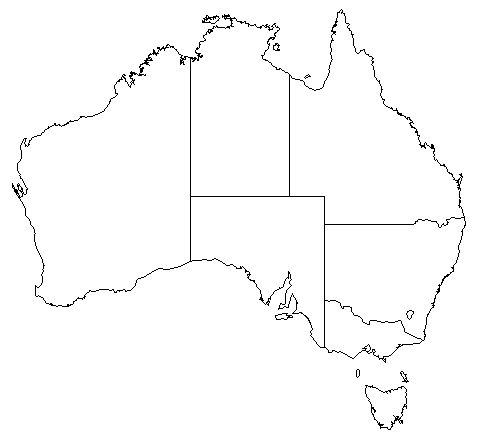
\includegraphics[width=.2\textwidth]{australia.pdf}}; \&[2mm]  
    \node(i2){
    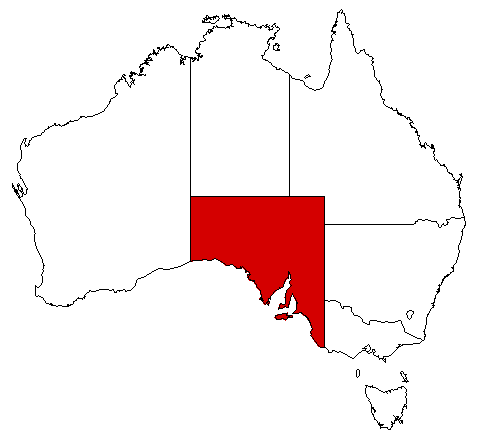
\includegraphics[width=.2\textwidth]{st-red.pdf}}; \&[2mm]
    \node(i3){
    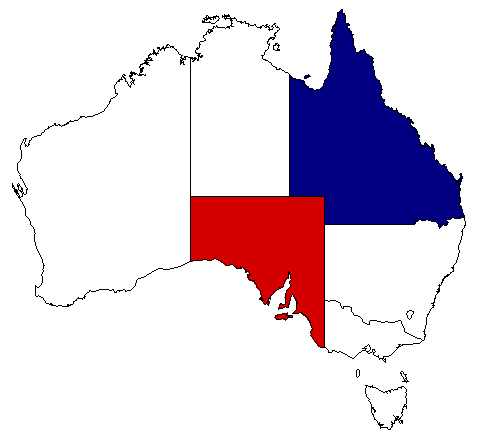
\includegraphics[width=.2\textwidth]{st-red-ql-blue.pdf}}; \&[2mm]
	\node(i4){
    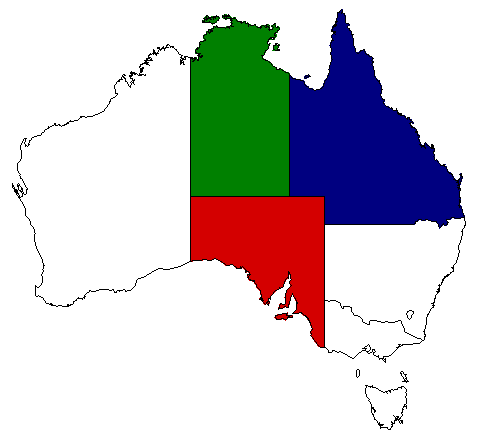
\includegraphics[width=.2\textwidth]{st-red-ql-blue-nt-green.pdf}};
    \\ 
	\node (l1) {Alle unbelegt}; \& 
	\node (l2) {SA in 5 Constraints}; \&
	\node(l3){$|D_\mathsf{QL}|$ nur 2 }; \&	
	\node(l4){$|D_\mathsf{NT}|$ nur 1 }; \&	
		
	\\
  };
  
\end{tikzpicture}
\end{frame}

\begin{frame}{Wertordnung}
Wähle die Belegung, die
die wenigsten Domäneneinschränkungen zur Folge haben.
\begin{center}
\begin{tikzpicture}[auto,
                    ->,>=stealth',shorten >=1pt,thick,
                    node distance=2.6cm,inner sep=0pt,
                    constraint/.style={circle,fill=black!15,draw,font=\sffamily\small}]
\node (1) at (0, 0)                   {
\def\svgwidth{.15\columnwidth}
\input{img/blue-red.pdf_tex}
};

\node[below left of=1] (2) {
\def\svgwidth{.15\columnwidth}
\input{img/wa-red-green.pdf_tex}

{\huge
\alert{\Lightning}
}
};  

\node[below right of=1] (3) {
\def\svgwidth{.15\columnwidth}
\input{img/wa-red-blue.pdf_tex}
};  


\node[below left of=2] (l2) {
Es bleibt \alert{kein} Wert für SA.
};

\node[below right of=3] (l3) {
Es bleibt ein Wert für SA.
};


\path[every node/.style={font=\sffamily\tiny}]
  (1) edge (2)
  (1) edge (3)
 ;
\end{tikzpicture}
\end{center}
\end{frame}